% from github:Latex-IEEE-Conferences-Chinese-master


\documentclass[10pt, conference, compsocconf]{IEEEtran}
\usepackage{CJKutf8}
\usepackage{cite}
\usepackage{amsmath,amssymb,amsfonts}
\usepackage{algorithmic}
\usepackage{graphicx}
\usepackage{textcomp}
%\usepackage{pythonhighlight}
\hyphenation{op-tical net-works semi-conduc-tor}

\begin{document}
	\begin{CJK}{UTF8}{gbsn}

\title{Assignment for Image Classification}

\author
{\IEEEauthorblockN{Qilei Li}
    \IEEEauthorblockA
    {
    EE\\
    四川大学\\
    成都, 中国\\
    qilei.li@foxmail.com
    }
}

\maketitle

\begin{abstract}
这里是摘要。
\end{abstract}


\IEEEpeerreviewmaketitle

\section{项目}
\begin{itemize}
	\item	项目1
	\item	项目2

	
\end{itemize}

\section{第一部分}
这里是第一部分


\begin{figure}[h]
	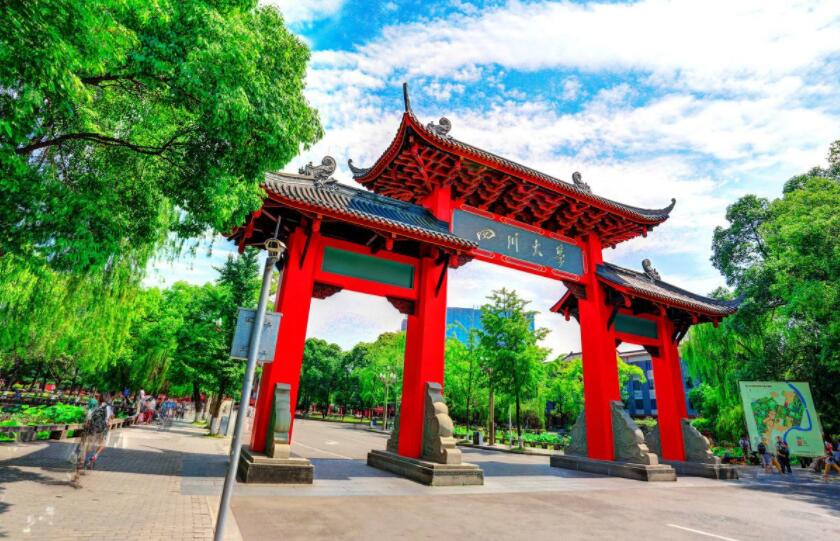
\includegraphics[width=8cm]{school.jpg}
	\caption{school} 
	\label{school}
\end{figure}




\subsection{小节}
可以导入代码
%需要引用第三方库
%\begin{python}
%import numpy as np
%a = np.random.randn((5,5))
%\end{python}



\subsubsection{小小节}

\begin{equation}
  E= MC^2
\end{equation}


\begin{equation}
max(0,x)=\left\{
\begin{aligned}
0, \quad x \leq 0 & \\
1, \quad x > 0  &
\end{aligned}
\right.
\end{equation}

参考文献的引用:
\cite{yearbook2005china}

\bibliographystyle{IEEEtran} 
\bibliography{ref}   



\end{CJK}
\end{document}